\documentclass[11pt,landscape]{article}
\usepackage[margin=10mm]{geometry}
\usepackage[T1]{fontenc}
\usepackage[utf8]{inputenc}
\usepackage{lmodern}
\usepackage{amsmath}
\usepackage{amssymb}
\usepackage{tikz}
\usetikzlibrary{arrows.meta, positioning, calc, backgrounds, fit}
\pagestyle{empty}

\begin{document}

\noindent\makebox[\textwidth][c]{\Large GRLNet: ConvLSTM Cell Internal View}

\vspace{2mm}

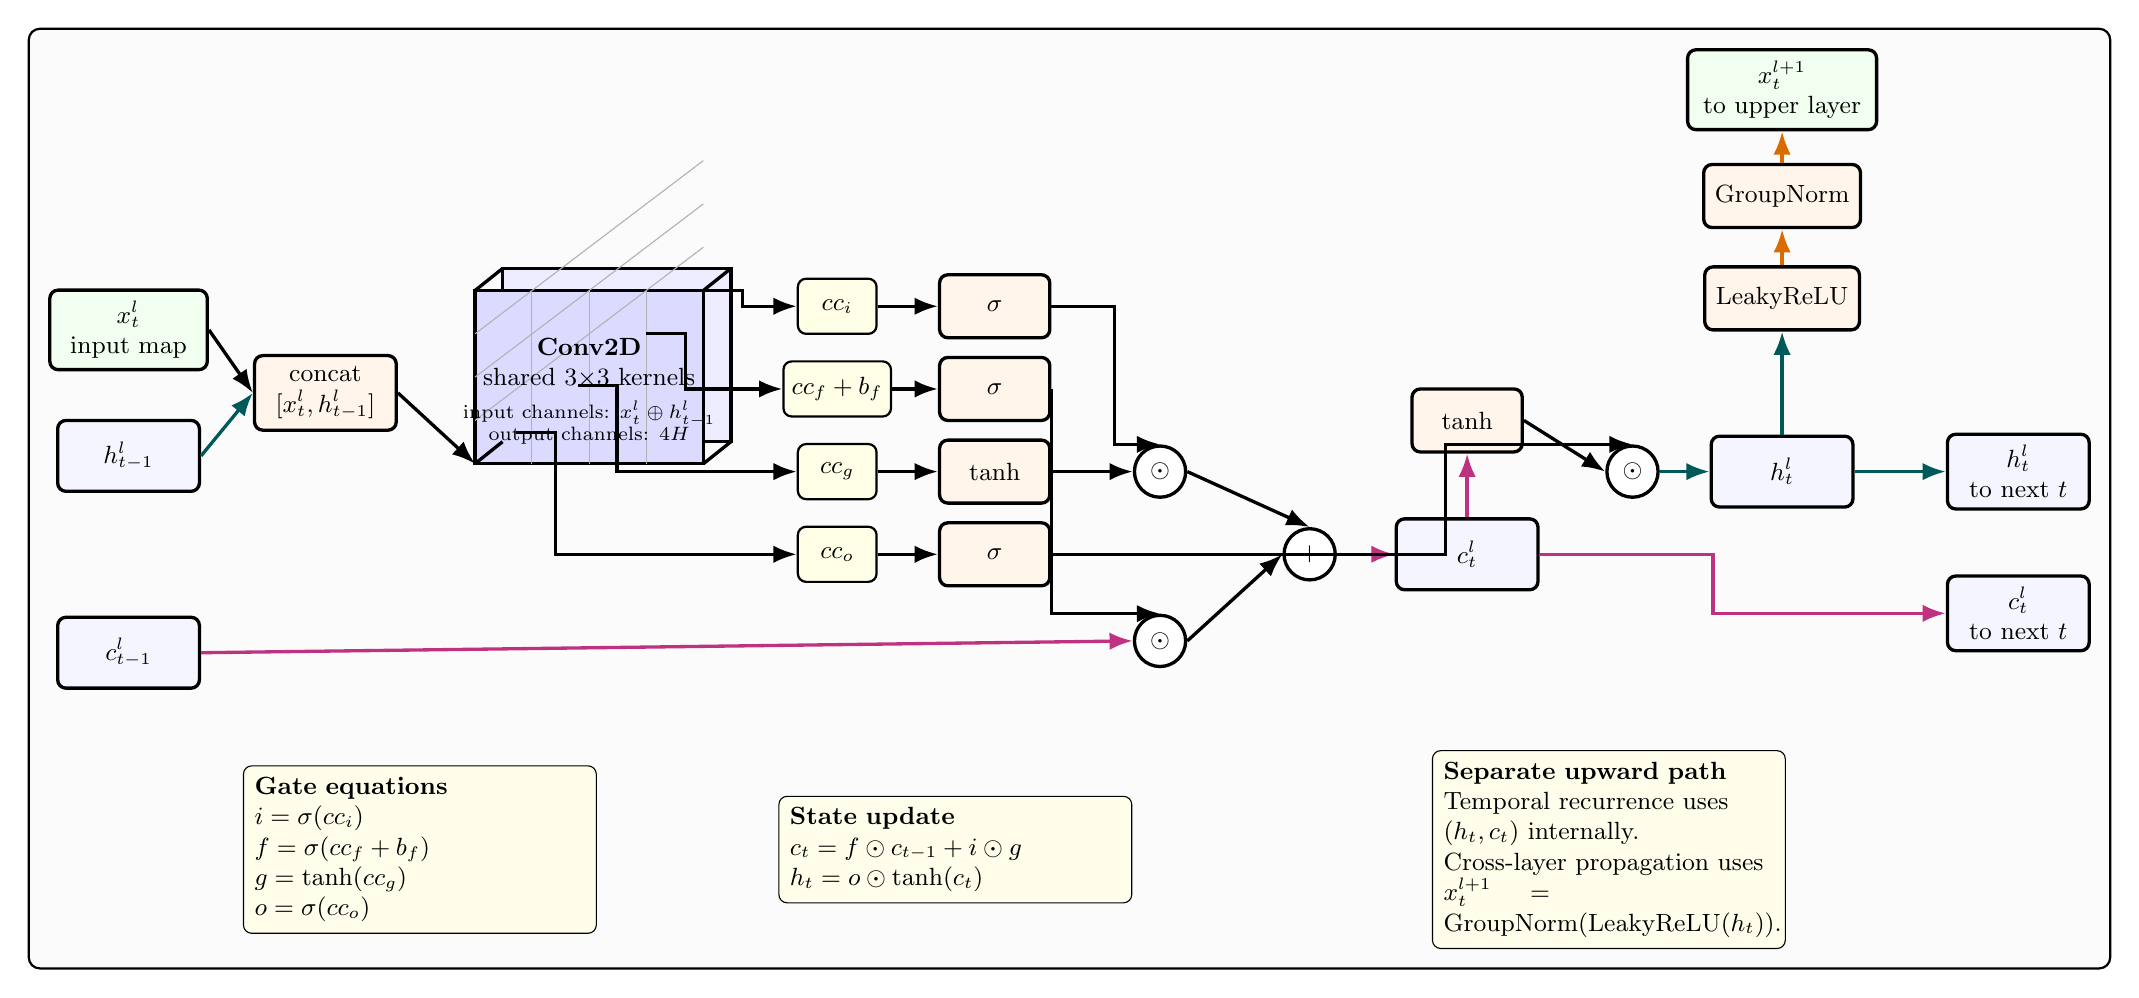
\begin{tikzpicture}[
    >=Latex,
    font=\small,
    io/.style={draw, rounded corners=3pt, very thick, align=center, inner sep=4pt, fill=green!6, minimum width=20mm, minimum height=9mm},
    op/.style={draw, rounded corners=3pt, very thick, align=center, inner sep=4pt, fill=orange!8, minimum width=14mm, minimum height=8mm},
    state/.style={draw, rounded corners=3pt, very thick, align=center, inner sep=4pt, fill=blue!4, minimum width=18mm, minimum height=9mm},
    gate/.style={draw, rounded corners=3pt, thick, align=center, inner sep=3pt, fill=yellow!10, minimum width=10mm, minimum height=7mm},
    note/.style={draw, rounded corners=3pt, align=left, inner sep=4pt, fill=yellow!8, text width=42mm, font=\small},
    hpath/.style={->, very thick, draw=teal!70!black},
    cpath/.style={->, very thick, draw=magenta!75!black},
    auxpath/.style={->, very thick, draw=orange!85!black},
    main/.style={->, very thick},
    sum/.style={circle, draw, very thick, fill=white, minimum size=6.5mm, inner sep=0pt},
    prod/.style={circle, draw, very thick, fill=white, minimum size=6.5mm, inner sep=0pt}
]

% Inputs
\node[io] (xin) at (0.0,1.7) {$x_t^l$\\input map};
\node[state] (hprev) at (0.0,0.1) {$h_{t-1}^l$};
\node[state] (cprev) at (0.0,-2.4) {$c_{t-1}^l$};

\node[op, minimum width=18mm] (concat) at (2.5,0.9) {concat\\$[x_t^l,h_{t-1}^l]$};
\draw[main] (xin.east) -- (concat.west);
\draw[hpath] (hprev.east) -- (concat.west);

% Conv box
\coordinate (convsw) at (4.4,0.0);
\coordinate (convne) at (7.3,2.2);
\def\dx{0.35}
\def\dy{0.28}
\draw[very thick, fill=blue!7] ($(convsw)+(\dx,\dy)$) rectangle ($(convne)+(\dx,\dy)$);
\draw[very thick, fill=blue!14] (convsw) rectangle (convne);
\draw[very thick] (convsw) -- ($(convsw)+(\dx,\dy)$);
\draw[very thick] (convne) -- ($(convne)+(\dx,\dy)$);
\draw[very thick] ($(convsw)+(0,2.2)$) -- ($(convsw)+(0,2.2)+(\dx,\dy)$);
\draw[very thick] ($(convsw)+(2.9,0)$) -- ($(convsw)+(2.9,0)+(\dx,\dy)$);
\foreach \yy in {0.55,1.10,1.65} {
  \draw[thin, gray!60] ($(convsw)+(0,\yy)$) -- ($(convne)+(0,\yy)$);
}
\foreach \xx in {0.72,1.45,2.18} {
  \draw[thin, gray!60] ($(convsw)+(\xx,0)$) -- ($(convsw)+(\xx,2.2)$);
}
\node[align=center] at ($(convsw)!0.5!(convne)+(0,0.18)$) {\textbf{Conv2D}\\shared $3{\times}3$ kernels};
\node[font=\scriptsize, align=center] at ($(convsw)!0.5!(convne)+(0,-0.58)$) {input channels: $x_t^l \oplus h_{t-1}^l$\\output channels: $4H$};
\draw[main] (concat.east) -- (convsw);

% Split to four gate preactivations
\node[gate] (cci) at (9.0,2.0) {$cc_i$};
\node[gate] (ccf) at (9.0,0.95) {$cc_f+b_f$};
\node[gate] (ccg) at (9.0,-0.10) {$cc_g$};
\node[gate] (cco) at (9.0,-1.15) {$cc_o$};
\draw[main] (convne) -- ++(0.5,0) |- (cci.west);
\draw[main] ($(convsw)!0.75!(convne)$) -- ++(0.5,0) |- (ccf.west);
\draw[main] ($(convsw)!0.45!(convne)$) -- ++(0.5,0) |- (ccg.west);
\draw[main] ($(convsw)!0.18!(convne)$) -- ++(0.5,0) |- (cco.west);

% Nonlinearities
\node[op] (gi) at (11.0,2.0) {$\sigma$};
\node[op] (gf) at (11.0,0.95) {$\sigma$};
\node[op] (gg) at (11.0,-0.10) {$\tanh$};
\node[op] (go) at (11.0,-1.15) {$\sigma$};
\draw[main] (cci.east) -- (gi.west);
\draw[main] (ccf.east) -- (gf.west);
\draw[main] (ccg.east) -- (gg.west);
\draw[main] (cco.east) -- (go.west);

% Cell update
\node[prod] (mulf) at (13.1,-2.25) {$\odot$};
\node[prod] (muli) at (13.1,-0.10) {$\odot$};
\node[sum]  (sumc) at (15.0,-1.15) {$+$};
\node[state] (ct) at (17.0,-1.15) {$c_t^l$};

\draw[cpath] (cprev.east) -- (mulf.west);
\draw[main] (gf.east) |- (mulf.north);
\draw[main] (gi.east) -- ++(0.8,0) |- (muli.north);
\draw[main] (gg.east) -- (muli.west);
\draw[main] (mulf.east) -- (sumc.west);
\draw[main] (muli.east) -- (sumc.north);
\draw[cpath] (sumc.east) -- (ct.west);

% Hidden update
\node[op]   (tanhc) at (17.0,0.55) {$\tanh$};
\node[prod] (mulh)  at (19.1,-0.10) {$\odot$};
\node[state] (ht)   at (21.0,-0.10) {$h_t^l$};

\draw[cpath] (ct.north) -- (tanhc.south);
\draw[main] (tanhc.east) -- (mulh.west);
\draw[main] (go.east) -- ++(5.0,0) |- (mulh.north);
\draw[hpath] (mulh.east) -- (ht.west);

% Outputs: temporal and upward
\node[state] (hnext) at (24.0,-0.10) {$h_t^l$\\to next $t$};
\node[state] (cnext) at (24.0,-1.90) {$c_t^l$\\to next $t$};
\draw[hpath] (ht.east) -- (hnext.west);
\draw[cpath] (ct.east) -- ++(2.2,0) |- (cnext.west);

\node[op, minimum width=18mm] (lrelu) at (21.0,2.10) {LeakyReLU};
\node[op, minimum width=18mm] (gnorm) at (21.0,3.40) {GroupNorm};
\node[io, minimum width=24mm] (xup) at (21.0,4.75) {$x_t^{l+1}$\\to upper layer};
\draw[hpath] (ht.north) -- (lrelu.south);
\draw[auxpath] (lrelu.north) -- (gnorm.south);
\draw[auxpath] (gnorm.north) -- (xup.south);

% Notes
\node[note] (n1) at (3.7,-4.9) {
\textbf{Gate equations}\\
$i=\sigma(cc_i)$\\
$f=\sigma(cc_f+b_f)$\\
$g=\tanh(cc_g)$\\
$o=\sigma(cc_o)$
};

\node[note] (n2) at (10.5,-4.9) {
\textbf{State update}\\
$c_t=f \odot c_{t-1}+i \odot g$\\
$h_t=o \odot \tanh(c_t)$
};

\node[note] (n3) at (18.8,-4.9) {
\textbf{Separate upward path}\\
Temporal recurrence uses $(h_t,c_t)$ internally.\\
Cross-layer propagation uses\\
$x_t^{l+1}=\mathrm{GroupNorm}(\mathrm{LeakyReLU}(h_t))$.
};

\begin{scope}[on background layer]
    \node[draw, rounded corners=4pt, thick, fit=(xin)(hprev)(cprev)(concat)(xup)(hnext)(cnext)(n1)(n2)(n3), inner sep=7pt, fill=gray!3] {};
\end{scope}

\end{tikzpicture}

\end{document}
